\documentclass[12pt]{article}
\usepackage{amsthm,amssymb,amsmath,amsfonts}
\usepackage[a4paper, top=25mm, bottom=30mm, left=25mm, right=25mm]{geometry}
\usepackage[pagebackref=false,colorlinks,linkcolor=black,citecolor=black]{hyperref}
\usepackage[nameinlink]{cleveref}
 \AtBeginDocument{%
    \crefname{equation}{برابری}{equations}%
    \crefname{chapter}{فصل}{chapters}%
    \crefname{section}{بخش}{sections}%
    \crefname{appendix}{پیوست}{appendices}%
    \crefname{enumi}{مورد}{items}%
    \crefname{footnote}{زیرنویس}{footnotes}%
    \crefname{figure}{شکل}{figures}%
    \crefname{table}{جدول}{tables}%
    \crefname{theorem}{قضیه}{theorems}%
    \crefname{lemma}{لم}{lemmas}%
    \crefname{corollary}{نتیجه}{corollaries}%
    \crefname{proposition}{گزاره}{propositions}%
    \crefname{definition}{تعریف}{definitions}%
    \crefname{result}{نتیجه}{results}%
    \crefname{example}{مثال}{examples}%
    \crefname{remark}{نکته}{remarks}%
    \crefname{note}{یادداشت}{notes}%
    \crefname{observation}{مشاهده}{observations}%
    \crefname{algorithm}{الگوریتم}{algorithms}%
    \crefname{cproof}{برهان}{cproofs}%
}

\usepackage{tikz}
\usepackage{graphicx}
\usepackage{booktabs}
\usepackage{color}
\usepackage{graphicx}
\usepackage{subcaption}

\usepackage{setspace}
\doublespacing

\usepackage{titletoc}
\usepackage{tocloft}
\usepackage{enumitem}
\usepackage{amsmath, amssymb}
\usepackage{algorithm}
\usepackage[noend]{algorithmic}
\renewcommand{\algorithmicrequire}{\textbf{Input:}}
\renewcommand{\algorithmicensure}{\textbf{Output:}}

\usepackage{tabularx}
\makeatletter
\newcommand{\multiline}[1]{%
  \begin{tabularx}{\dimexpr\linewidth-\ALG@thistlm}[t]{@{}X@{}}
    #1
  \end{tabularx}
}
\makeatother

\usepackage{float}
\usepackage{verbatim}
\makeindex
\usepackage{sectsty}
\usepackage{xepersian}
\SepMark{-}
\settextfont[Scale=1.2,Path=fonts/,BoldFont=B Nazanin Bold.ttf]{B Nazanin.ttf}
\setlatintextfont{Times New Roman}
\renewcommand{\labelitemi}{$\bullet$}

\theoremstyle{definition}
\newtheorem{definition}{تعریف}[section]
\newtheorem{remark}[definition]{نکته}
\newtheorem{note}[definition]{یادداشت}
\newtheorem{example}[definition]{نمونه}
\newtheorem{question}[definition]{سوال}
\newtheorem{remember}[definition]{یاداوری}
\newtheorem{observation}[definition]{مشاهده}
\theoremstyle{theorem}
\newtheorem{theorem}[definition]{قضیه}
\newtheorem{lemma}[definition]{لم}
\newtheorem{proposition}[definition]{گزاره}
\newtheorem{corollary}[definition]{نتیجه}
\newtheorem*{cproof}{برهان}




\begin{document}
\fontsize{12pt}{14pt}\selectfont

\begin{minipage}{0.1\textwidth}

\includegraphics[width=3cm]{etc/IUST}
\end{minipage}%
\hfill%
\begin{minipage}{0.6\textwidth}\centering
\fontsize{13pt}{13pt}\selectfont
به‌ نام خدا \\
\textbf{درس یادگیری عمیق} \\
\textbf{تمرین سری ششم}\\
استاد درس : دکتر محمدرضا محمدی \\
دستیاران :  مهدی خورشا، سید محمد موسوی،\\ امیرحسین نمازی
\\
\vspace{0.25cm}
\begingroup
\fontsize{11pt}{11pt}\selectfont
دانشگاه علم و صنعت ایران، دانشکده مهندسی کامپیوتر \\
نیمسال دوم تحصیلی 1403 - 1404 \\
\endgroup
\end{minipage}%
\hfill%
\begin{minipage}{0.1\textwidth}

\end{minipage}

\vspace{0.5cm}

\noindent\rule{\textwidth}{1pt}

\centering {\fontsize{18}{22}\selectfont \textbf{مهلت تحویل : 1404/03/20 }}\\
{\fontsize{14}{22}\selectfont \textbf{لطفا به نکات موجود در سند قوانین انجام و تحویل تمرین ها دقت فرمایید. }}

\begin{enumerate}

    \section*{سوالات تئوری}
    \item 
\includegraphics[width=1cm]{figs/Forbidden_AI.jpg}
    در این درس با \href{https://arxiv.org/pdf/2006.11239}{مدل های انتشار نویز زدایی}\LTRfootnote{DDPM} آشنا شدید.\\
    اکنون \href{https://arxiv.org/pdf/2006.09011}{مدل های‌امتیازی شرطی‌شده با نویز}\LTRfootnote{NCSN} را مطالعه کرده و به پرسش‌های زیر پاسخ دهید(۱۵ نمره):
    
    \begin{enumerate}
        \item روش را کوتاه توضیح داده و بگویید \lr{Langevin dynamics} چیست و چه کارکردی در آن دارد؟
        \item چگونه مدل‌های انتشار چالش فرض چندگانه و چگالی داده کم را برطرف می‌کنند؟
        \item 
    اندازه نویز افزوده شده و گام زمانی چه تاثیری در مدل‌های انتشار دارد?برای مثال اگر به جای 40 مرحله نویز تنها 3 گام نویز ولی با اندازه بیشتری افزوده شود یا برعکس 80 گام نویز با اندازه کمتری افزوده شود، هر کدام چه برتری و کاستی‌هایی دارد؟
    \end{enumerate}

     
    \item 
\includegraphics[width=1cm]{figs/Forbidden_AI.jpg}
    
    \lr{WGAN}، که در این \href{https://arxiv.org/pdf/1701.07875}{مقاله} معرفی شد، یکی از اولین گام‌های بزرگ به سوی پایدارسازی آموزش \lr{GAN} بود. با چند تغییر، نویسندگان توانستند نشان دهند چگونه می‌توان \lr{GAN‌} هایی را آموزش داد که دارای دو ویژگی زیر باشند:
    
    \begin{itemize}
      \item یک معیار ضرر معنادار که با همگرایی \lr{generator} و کیفیت نمونه‌ها همبستگی دارد.
      \item بهبود پایداری فرآیند بهینه‌سازی. به طور خاص، این مقاله تابع ضرر واسرشتاین را برای هر دو \lr{discriminator} و \lr{generator} معرفی می‌کند. استفاده از این تابع ضرر به جای \lr{binary cross-entropy} منجر به همگرایی پایدارتر \lr{GAN} می‌شود.
    \end{itemize}
    
    در بسیاری از موارد، الگوریتم \lr{GAN} می‌تواند به عنوان کمینه‌سازی انحراف بین توزیع داده‌ها \( p_{\text{\lr{data}}} \) و توزیع مدل \( p_g \) در نظر گرفته شود. در این مسئله، ما یک مشکل با انحراف‌های مختلف (مثلاً انحراف \lr{Jensen-Shannon} و انحراف \lr{KL}) و یک راه‌حل بالقوه برای رفع آن (\lr{Wasserstein Distance}) را بررسی خواهیم کرد(۲۰ نمره).
    
    \begin{enumerate}
        \item[الف)] فرض کنید \( p_{\text{\lr{data}}} \sim \mathcal{N}(\theta_0, \epsilon^2) \) و \( p_g \sim \mathcal{N}(\theta, \epsilon^2) \) توزیع‌های نرمال با انحراف معیار \( \epsilon \) باشند که به ترتیب حول \( \theta_0 \in \mathbb{R} \) و \( \theta \in \mathbb{R} \) مرکزیت دارند. نشان دهید که:
        \[
        D_{\text{\lr{KL}}}(p_g \,\|\, p_{\text{\lr{data}}}) = \frac{(\theta - \theta_0)^2}{2\epsilon^2}
        \]
    
        \item[ب)] فرض کنید \( p_{\text{\lr{data}}} \) و \( p_g \) هر دو جرم احتمال را فقط در یک بخش بسیار کوچک از دامنه داشته باشند؛ یعنی، حد \( \epsilon \rightarrow 0 \). چه اتفاقی برای \( D_{\text{\lr{KL}}}(p_g \,\|\, p_{\text{\lr{data}}}) \) و مشتق آن نسبت به \( \theta \)، با فرض اینکه \( \theta \ne \theta_0 \)، می‌افتد؟
    
        \item[ج)] آیا این امر مشکلی برای یک \lr{GAN} که با تابع ضرر تعریف‌شده‌ی زیر آموزش داده شده‌ باشد، ایجاد می‌کند؟ چرا؟
        \[
        L_G(\theta; \phi) = \mathbb{E}_{x \sim p_\theta(x)}[\log(1 - D_\phi(x))] - \mathbb{E}_{x \sim p_\theta(x)}[\log D_\phi(x)]
        \]
    
        \item[د)] تحت همان شرایط (ب)، انحراف \lr{KL}، انحراف \lr{JS} و فاصله واسرشتاین را مقایسه کنید.
    \end{enumerate}

    
    \item 
\includegraphics[width=1cm]{figs/Forbidden_AI.jpg}
    در ارتباط با \lr{DDPM} به سوالات زیر پاسخ دهید(۲۰ نمره):
    \begin{enumerate}
    \item فرض کنید $x_{t}$ متغیر تصادفی(یک نمونه داده مثلا یک تصویر)‌ای است که در فرایند \lr{Forward Diffusion Process} با اضافه شدن مقداری نویز به $x_{t-1}$ بدست می‌آید. بر این اساس عبارت زیر را توضیح دهید:
    $$
    x_t = \sqrt{1 - \beta_t} \, x_{t-1} + \sqrt{\beta_t} \, \epsilon
    $$
    \item با استفاده از ترفند تغییر پارامتر\LTRfootnote{Reparameterization trick} نشان دهید عبارت قسمت (آ) را می‌توان بصورت زیر نوشت:\\
    $$
    x_t = \sqrt{\bar{\alpha}_t} \, x_0 + \sqrt{1 - \bar{\alpha}_t} \, \epsilon
    $$
    \item با توجه به شکل \ref{fig:q4}  توضیح دهید که چرا به هنگام حذف نویز از داده در فرایند \lr{Reverse Diffusion Process} در هر مرحله نمی‌توانیم به طور مستقیم نویز را حذف کنیم(از $x_{t}$ به $x_{t-1}$ برسیم) و چرا این عمل برایمان غیرقابل حل \LTRfootnote{intractable}می‌باشد؟ (با توجه به شکل \ref{fig:q4} این امر موجب می‌شود تا از روش‌های تخمین تابع مانند شبکه‌های عصبی استفاده کنیم.)
    \begin{figure}[ht]
        \centering
        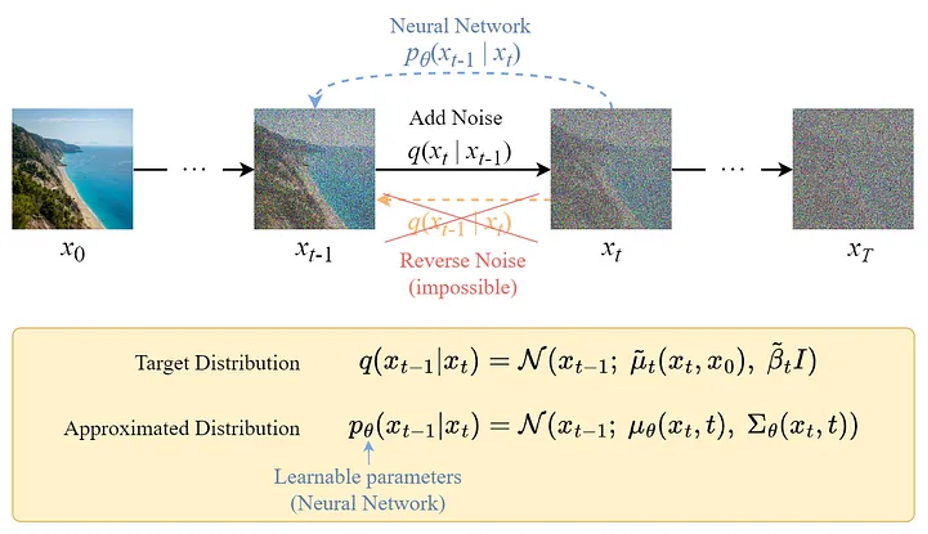
\includegraphics[width=0.85\textwidth]{figs/Q4.png}
        \caption{تابع توزیع تخمین‌زده‌شده توسط شبکه‌ی عصبی}
        \label{fig:q4}  
    \end{figure}

    \item تحقیق کنید که چه ویژگی‌هایی از مدل \lr{U-Net} موجب شد که نویسندگان مقاله \lr{DDPM} از آن برای معماری کار خود استفاده کنند؟
    \end{enumerate}
    
    \section*{سوالات عملی} 
    \item 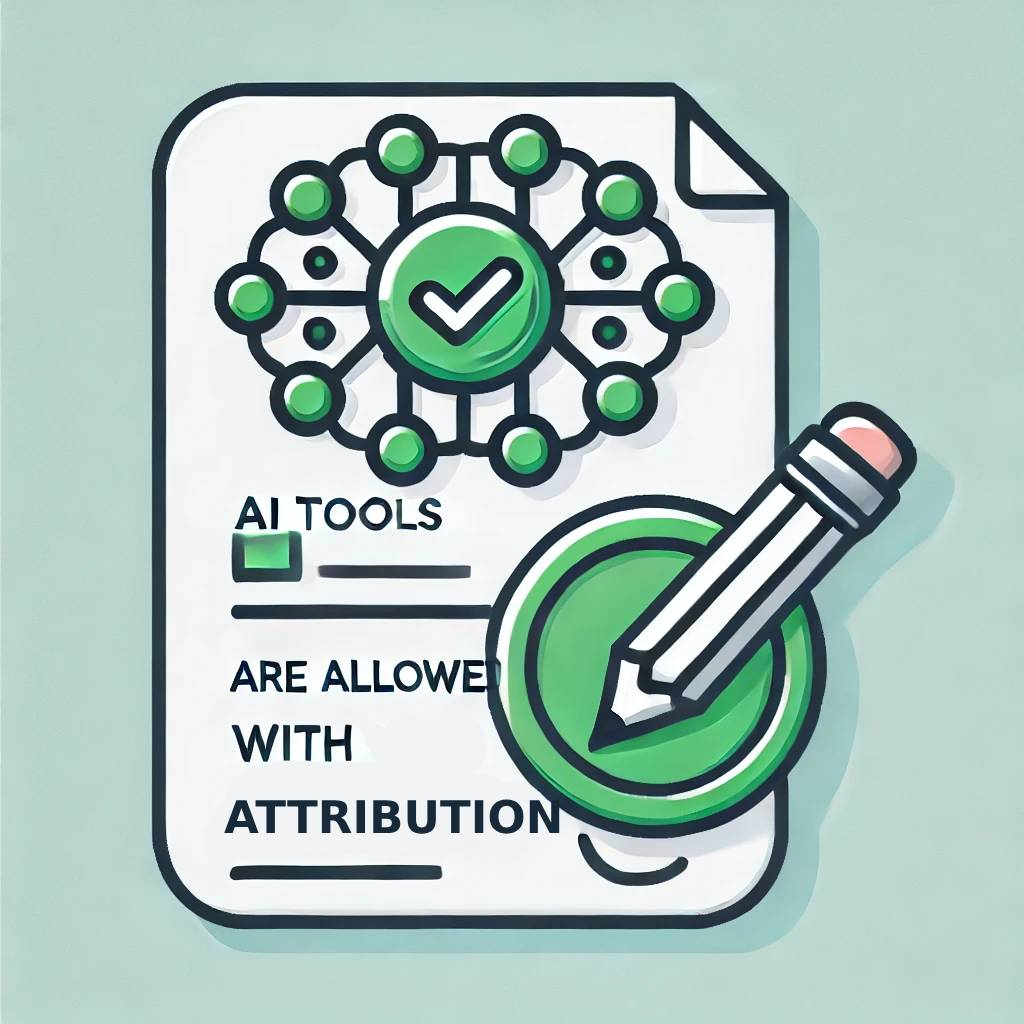
\includegraphics[width=1cm]{figs/Allowed_with_contributino.jpg}
    به این \href{https://github.com/dome272/Diffusion-Models-pytorch}{لینک گیت‌هاب} رفته و به پرسش‌های زیر پاسخ دهید(۲۵ نمره).
    \begin{enumerate}
        \item درباره هدایت بدون دسته‌بند مطالعه کرده و بگویید در کجای کد از آن استفاده شده است؟
        \item شرط در مدل انتشار شرطی به چه شکل اعمال شده است؟ آیا تنها به همین روش می‌توان شرط را اعمال کرد؟ اگر خیر، روش‌های دیگر چیست؟
        \item فرض کنید شرط ما متن باشد و راهنمای بدون طبقه‌بندی را به شکل زیر استفاده کنیم:
        $$
        text_{-}embeddings = text_{-}encoder(["", prompt])
        $$
        کد را بر این اساس تغییر بدهید و بگویید کدام ماژول‌ها تغییر می‌کنند.
        \item  \lr{stable diffusion} چیست؟ کد را براساس آن تغییر دهید و بگویید کدام ماژول‌ها تغییر می‌کنند.

    \end{enumerate}




    
    \item 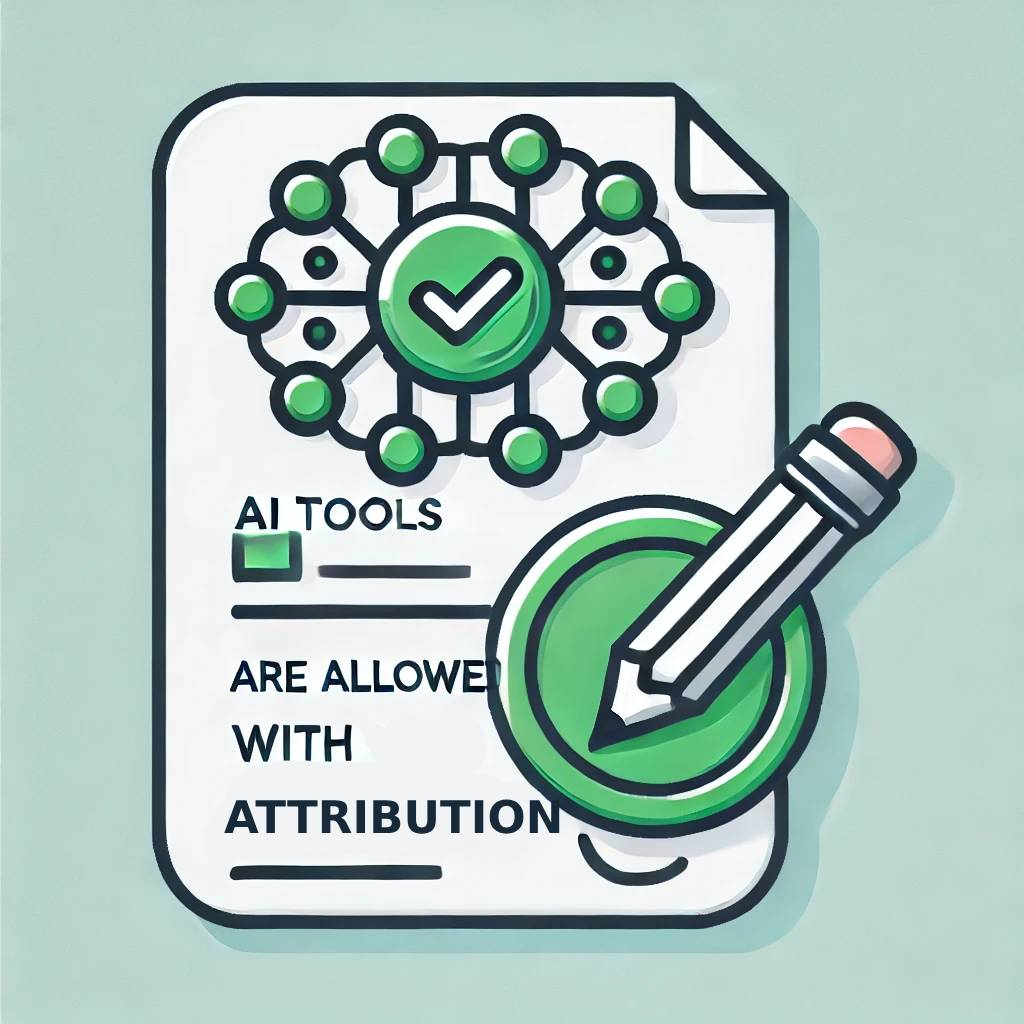
\includegraphics[width=1cm]{figs/Allowed_with_contributino.jpg}
     در این تمرین، شما قرار است دو مدل مولد مهم در یادگیری ماشین را روی مجموعه داده‌ی \lr{MNIST} پیاده‌سازی کنید: خودرمزگذار متغیر (\lr{VAE}) و شبکه مولد تخاصمی (\lr{GAN})(۲۰ نمره).\\
    مدل‌های \lr{VAE} یک متغیر پنهان احتمالاتی را از داده‌های ورودی یاد می‌گیرند، سپس از روی این توزیع نمونه‌برداری کرده و داده‌های جدیدی تولید می‌کنند.\\
    مدل‌های \lr{GAN} از یک شبکه مولد برای تولید تصاویر استفاده می‌کنند که توزیع آن‌ها به توزیع داده‌های واقعی نزدیک است.\\
   نوتبوک \lr{GAN-VAE.ipynb} حاوی کدهایی است که برخی بخش‌های آن با برچسب \lr{TODO} مشخص شده‌اند. شما باید این بخش‌ها را با دقت تکمیل کنید تا مدل‌ها به درستی پیاده‌سازی شوند.\\
    پیشنهاد می‌شود پیش از نوشتن کد، تمامی توضیحات و سلول‌ها را به‌دقت مطالعه کنید تا درک کاملی از ساختار مدل‌ها و نحوه پیاده‌سازی آن‌ها داشته باشید.

     \item 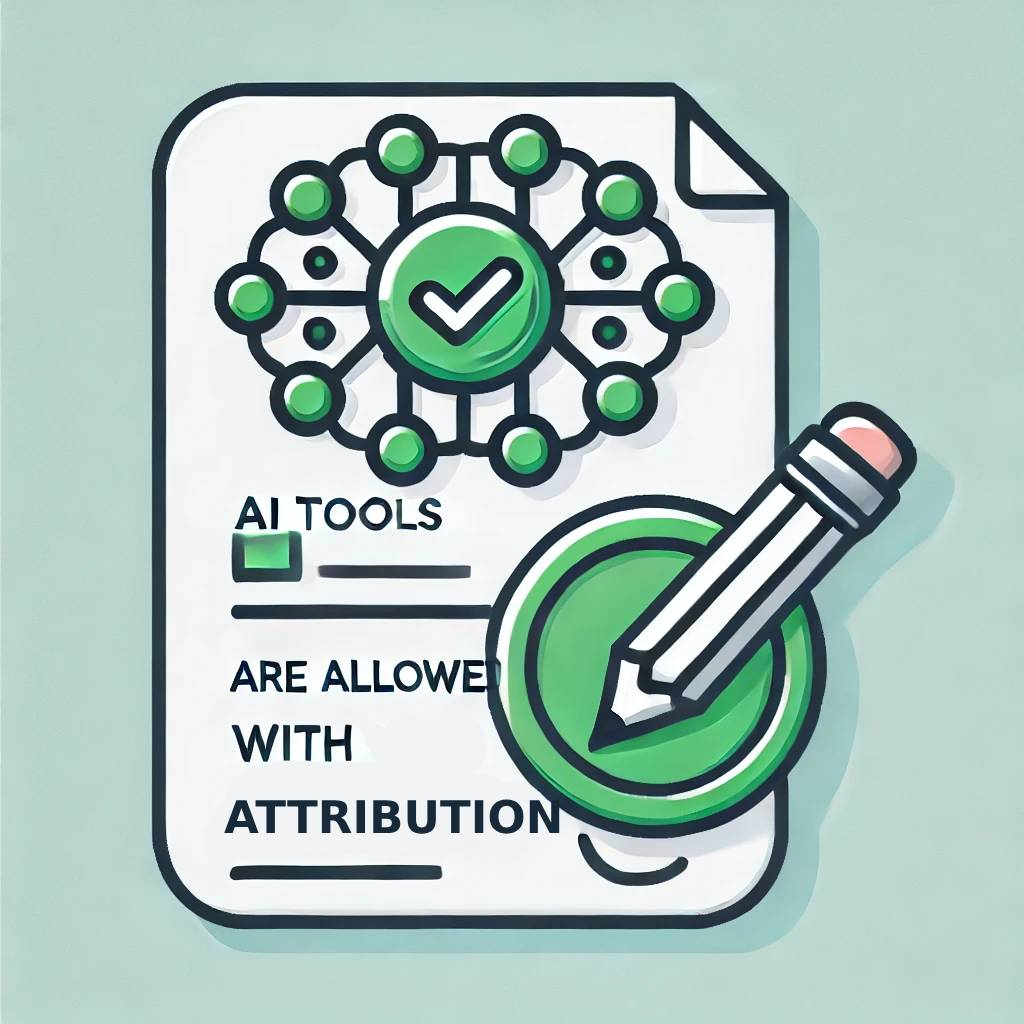
\includegraphics[width=1cm]{figs/Allowed_with_contributino.jpg}
     در این تمرین، هدف شما پیاده‌سازی یک مدل احتمالی انتشار نویز است. برای درک بهتر مفاهیم، توصیه می‌شود مقاله اصلی مربوط به \href{https://arxiv.org/pdf/2006.11239}{\lr{DDPM}} را مطالعه کنید(۲۰ نمره).

    شما باید نوتبوک \lr{DDPM.ipynb} را تکمیل کرده و تمام سلول‌های آن را اجرا کنید. بخش‌هایی که نیاز به تکمیل دارند، با برچسب \lr{TODO} در داخل بلوک‌های کد مشخص شده‌اند.\\
    پیش از شروع به نوشتن کد، تمام توضیحات متنی و کدهای داده‌شده را با دقت بخوانید.\\
    این نوت‌بوک با استفاده از محیط‌های رایگان \lr{Google Colab} و \lr{Kaggle} آزمایش شده است؛ می‌توانید از این پلتفرم‌ها برای اجرای کدهای خود استفاده کنید.\\
    اطمینان حاصل کنید که تمامی سلول‌ها بدون خطا اجرا می‌شوند و عملکرد مورد انتظار را ارائه می‌دهند.\\

\end{enumerate}



\end{document}


